%This file will discuss project results (validation of solution)
%This file should be included in doc using \input{file}

\section{Project Results}

\subsection{Simulations}
\subsection{Hover Test}
Using the models and systems discussed in the previous subsection, our preliminary flight simulation was constructed.  The SimuLink model Dynamic\_Simulation.slx was created.  The altitude controller was tested by providing a step input.  After some tuning of the controller, we were able to obtain the following step response.

\begin{figure}[h]
	\centering
	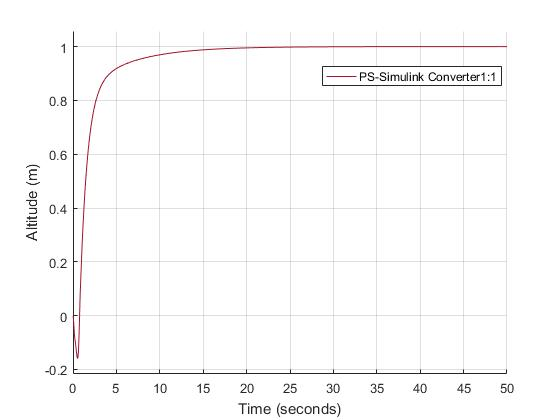
\includegraphics[scale = 0.5]{stepresponse.jpg}
	\caption{Hovering Step Response, for 1 metre altitude.}
	\label{fig:1m_step}
\end{figure}

When this test was initially performed, the SimScape MultiBody physical simulation did not yet include a model for a hard stop at the origin of the Z axis.  This is to say that there was no representation of ground for the quad-rotor drone to rest upon.  This is why an initial decline in position can be seen in the graph.  This was subsequently added this term.

Further tests to be performed during the week will outlined in Section \ref{discussion:sim}.



\subsection{Physical Implementation}

  To date, several tests and proof of concepts have been performed to determine methods of controlling hardware, limitations of the hardware or software and to determine feasibility of communication protocols. The test subjects include:
  
\begin{itemize}
  \item{Electronic Speed Controller}
  \item{Motor Lift Characteristics}
  \item{Wi-Fi Range}
  \item{Communication Channel}
  \item{Inertial Measurement Unit}
  \item{Miscellaneous Code Testing}
 \end{itemize}

  \subsubsection{Electronic Speed Controller}
  
The Afro ESC 12Amp BEC UltraLite Multirotor ESC V3 was tested at St. Mary's University with the assistance of Dr. Rhinelander. An Arduino running a script to map a potentiometer to a PWM duty cycle was used as an attempt to control the motor through the ESC. A 12V power supply fed the ESC while the Arduino controlled the duty cycle of the speed controller producing a voltage output to control the motor speed. 

The ESC testing was successful, the testing proved the Arduino's capability to control the motor with a variable input. The testing had flaws as a PWM duty cycle was used instead of a timed pulse width input. The duty cycle had potential of operating correctly as the range of times could have been calibrated to a range in the duty cycle although this method proved to be difficult due to low values causing the ESC to enter calibration mode. The script used to operate the ESC was re-written as a timed pulse width to ensure complete compatibility and ease of future integration.The pulse width script was tested using the ESC and was successful. The provided motor was successfully driven under no load conditions for the full range of pulse width values.

 \subsubsection{Motor Lift Characteristics}
 
 Using a 12V power supply, the provided ESC and the Multi-Star Elite motor the characteristics of the motor's lifting capacity were tested. A weight was attached to a support system with the motor and blade seated on top. The apparatus was placed on a scale and the scale's reading was zeroed. As the rotor speed increased, the reduction in weight read by the scale was considered the lift capacity.
 
 The test was performed beginning at a pulse width of 1127$\mu$s which was found through experimentation to be the cut in pulse width for motor operation. The test was performed at increments of 25$\mu$s. The resultant current draw values and lift values were documented. The lift values were used to create a simulink lookup table to characterize the motor's available force for simulation purposes. 
 
 During the load testing, it was noticed that the current draw from the individual motor was high. The power supply being used had a current limit of 3A therefore the maximum current draw allowed during testing was 2.95A to ensure no brown out due to lack of supply. The current limiting factor resulted in the test ending at a pulse width of 1525$\mu$s and a lift value of 137.5g.The resulting plot of the load testing is found in Figure \ref{fig:Motor_Char}.
 
 \begin{figure}{H}
	\centering
	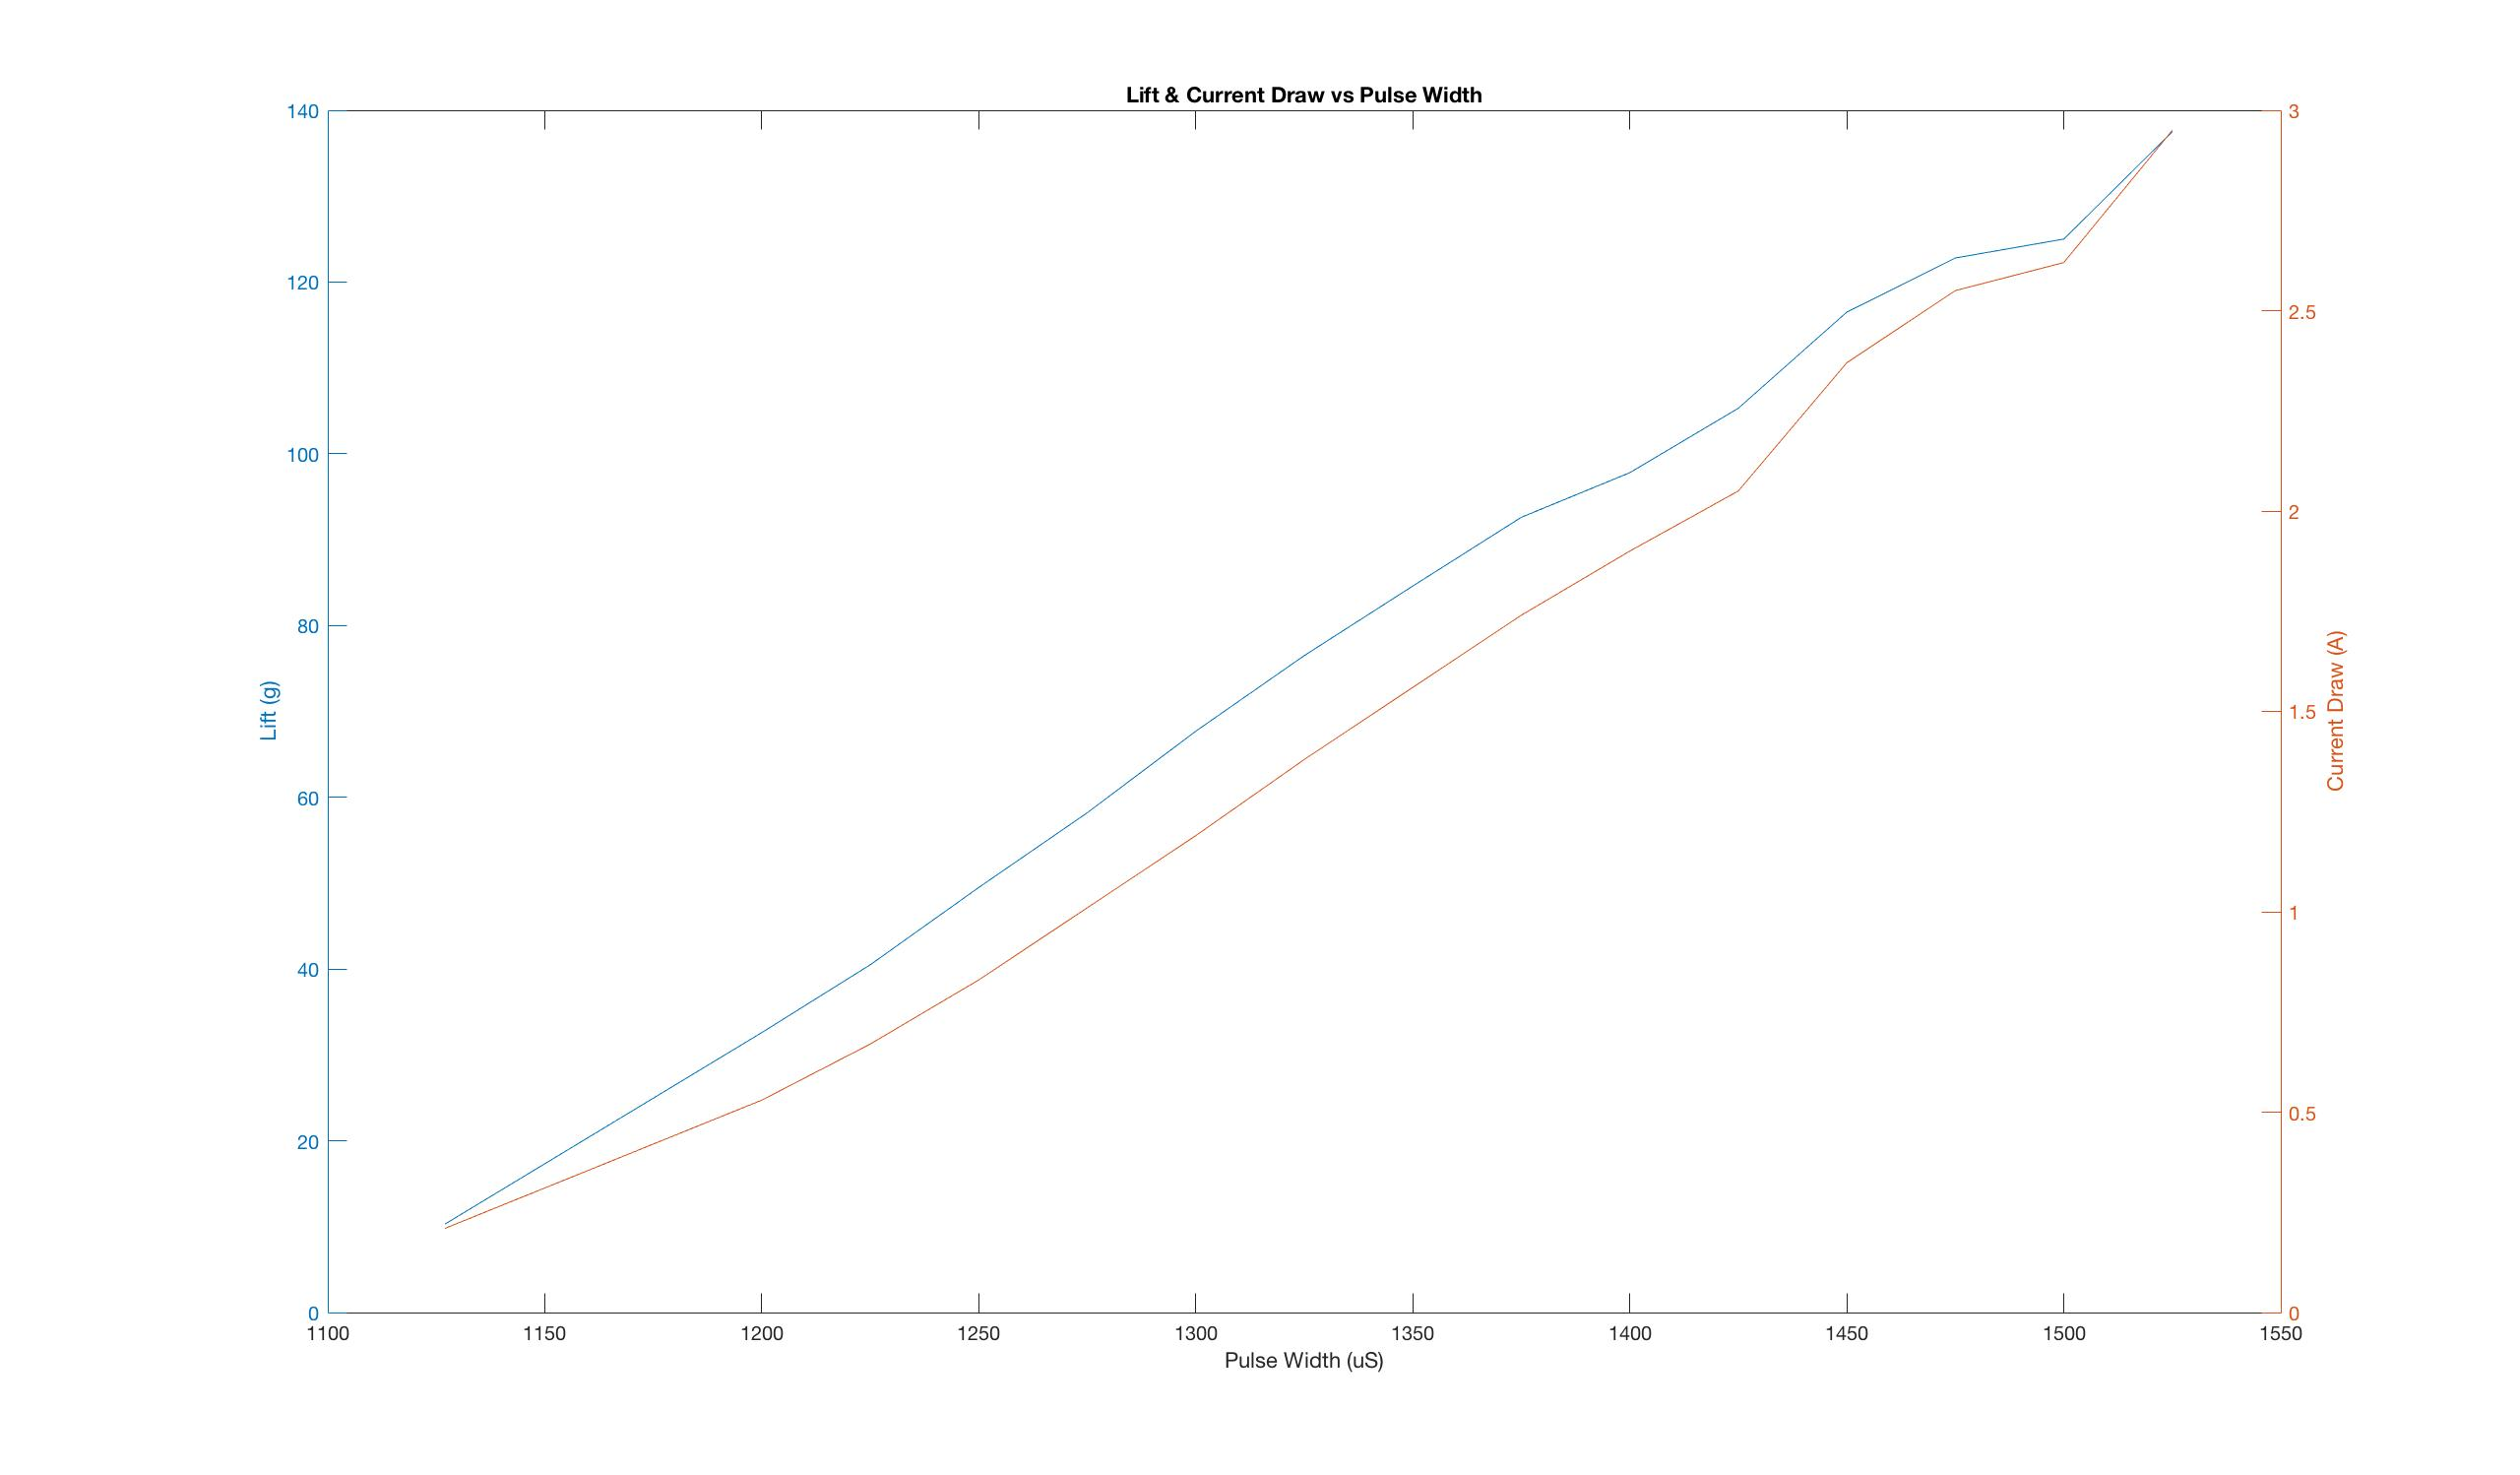
\includegraphics[width=1\textwidth]{Motor_Characterization.jpg}
	\caption{Motor Characterization Testing}
	\label{fig:Motor_Char}
\end{figure}

  \subsubsection{Wi-Fi and Bluetooth Range}
  
  A simple proof of concept regarding the range of Wi-Fi communications was performed. The test incorporated a a Wi-Fi communicating camera tethered to a Wi-Fi output from a cell phone. A user walked down Spring Garden holding the cell phone and found the approximate distance at which the phone and the camera lost communication. It was found that the range was approximately 100 ft with line of sight available with no Wi-Fi boosting technology. Bluetooth communications were also tested using the Raspberry Pi 3 connected to a Playstation 4 controller although the communication channel held a strong connection for only approximately 10 ft, this distance was considered insufficient for the scope of the project.
  
 \subsubsection{Communication Channel Testing}
 
 Several tests to ensure the communication channels were operating correctly were performed. Testing of each communicating device were performed while scripting but an overall test was performed to be sure data was being transmitted from the joystick control input, through the Wi-Fi connection, over serial to the Arduino and finally writing to the ESCs. The testing of the channel was performed by use of an LCD screen connected to the Arduino, with the values received by the Arduino being written to the screen. Most recent testing produced slightly unexpected results, as the joystick controller seemed to have the control inputs mapped incorrectly. The test was considered successful as the altitude input performed as expected. Remapping of control inputs is required. 

\subsubsection{Inertial Measurement Unit Testing}

The IMU was implemented and tested thoroughly for yaw, pitch, roll and altitude values. Altitude calculations were determined to be approximately +/- 50 cm in error without any filtering implemented. With an averaging filter implemented for the initial barometric pressure reading and a Kalman filter with feedback, the error was reduced to +/- 30 cm. Further filtering and testing of the altitude readings is to be performed. At low altitudes, +/- 30 cm error is considered too large as the stabilization PID loop will have difficulties when attempting to take off and land. Other measurement devices for low altitudes are going to be implemented and tested.

\subsubsection{Miscellaneous Testing}

All functions and scripts were tested to ensure compilation was possible and the program behaves as expected. Several tests and adjustments will be performed to ensure the device operates as expected prior to the submission of the final report. 



\subsection{Graphical User Interface}
The main validation for the GUI was to ensure that each of the push buttons do the proper thing as well as when a page is selected from the list widget that the proper page is displayed. The testing involved with this was to select the desired push button or page and ensure the expected outcome happens. Along this process many software bugs were encountered and fixed, these included invalid syntax, improper use of libraries and just wrong implementation. Through these tests much was learned and the result was a GUI that provides all of the required functionality and is intuitive. After these were validated testing the live plotting capability was next. 
\subsubsection{Live Plotting Testing}
Due to the new drone regulations proper flight tests to receive sensor data to live plot the altitude was unable to be performed. Instead, to validate that the plot on the seen in Figure \ref{fig:plot2} would update when new sensor data was received a test was developed. The test was to pull in data from a text file that was given in the form of x and y coordinates and then add new data to the text file as the GUI was running and make sure that the plot updated only when new data was availble. The definition to pull in the data from the file can be found in the liveData() definition in the GUI code in APPENDIX.

The result of this test was positive, whenever new data when entered into the text file plot would update to include to new data point accurately and swiftly. A flaw with this test could be that when the sensor data is receieved it would not come in this form, in this case the script would have to be altered to allow for a different data form. This test proved that the plot can be updated in real time.

